\documentclass[preprint]{elsarticle}
% 
% 
% 
% 
% 
% 
% 
% 
% 
\usepackage[a4paper, top=20mm, left =20mm, right =20mm ,bottom=20mm ]{geometry}
\usepackage{lineno}
\modulolinenumbers[1]
\journal{TRE}
\usepackage{graphicx}
\usepackage{ulem}
\usepackage{array}
\usepackage{epstopdf}
\usepackage{amstext}
\usepackage[utf8]{inputenc}
\usepackage[english]{babel}
\usepackage{amsfonts}
\usepackage{color}
\usepackage{amssymb}
\usepackage[citecolor=blue,linkcolor=blue,colorlinks=true]{hyperref}
\usepackage{multirow}
\usepackage{amsmath}
%\usepackage{lmodern}
%\usepackage{booktabs}
\usepackage{float}
\usepackage{tabularx}
\usepackage{geometry}
\usepackage{lscape}
\usepackage{longtable}
\usepackage{romannum}
\usepackage{makecell}
\usepackage{adjustbox}
\usepackage{lscape} 
%\usepackage{hyperref}

\usepackage{booktabs}

\usepackage{cleveref}
\usepackage{tablefootnote}
\crefformat{footnote}{#2\footnotemark[#1]#3}
\usepackage{blindtext}
\usepackage{algorithmicx,algpseudocode}
\usepackage[linesnumbered,ruled]{algorithm2e}
\usepackage{amsthm} % add by zhou
\newtheorem{theorem}{Theorem} % add by zhou
 
%\usepackage{longtable}
%\usepackage{natbib} 
%\usepackage[super,square]{natbib} 
\usepackage{longtable} 
\usepackage{float}
\usepackage{footnote}
\renewcommand{\thefootnote}{\arabic{footnote}}
%\pagenumbering{Roman} 
\pagenumbering{arabic} 
\newtheorem{definition}{Definition}
%\newcommand{\red}[1]{\textcolor{red}{#1}}
%%%%%%%%%%%%%%%%%%%%%%%
%% Elsevier bibliography styles
%%%%%%%%%%%%%%%%%%%%%%%
%% To change the style, put a % in front of the second line of the current style and
%% remove the % from the second line of the style you would like to use.
%%%%%%%%%%%%%%%%%%%%%%%
%% Numbered
%\bibliographystyle{model1-num-names}

%% Numbered without titles
%\bibliographystyle{model1a-num-names}

%% Harvard
% \bibliographystyle{model2-names.bst}\biboptions{authoryear}
%% Vancouver numbered
%\usepackage{numcompress}\bibliographystyle{model3-num-names}

%% Vancouver name/year
%\usepackage{numcompress}\bibliographystyle{model4-names}\biboptions{authoryear}

%% APA style
%\bibliographystyle{model5-names}
%\biboptions{authoryear}
%\bibliographystyle{apa}
%% AMA style
%\usepackage{numcompress}\bibliographystyle{model6-num-names}

%% `Elsevier LaTeX' style
%\bibliographystyle{elsarticle-num}
%%%%%%%%%%%%%%%%%%%%%%%
%\bibliographystyle{apalike}
\newlength\mylength
\renewcommand{\baselinestretch}{1.5}
% 
% 
% 
% 
% 
% 
% 
% 
% 
% 
% 
% 
% 

% 
% 
\begin{document}
\linenumbers
\begin{frontmatter}
    \title{An AI-based conceptual framework for port ranking}

    \author[1]{Yanjie Zhou}
    \author[1]{Xiaojin Wang}
    \author[2]{Zehao Qian}
    \author[1]{Tao Li}
    % 
    % 
    % 
    \cortext[cor1]{Author to whom correspondence should be addressed.}
    \address[1]{School of Management, Zhengzhou University,  China, 315100, China}
    \address[2]{Department of Nature Sciences, Durham University, UK, DH1 3LE}

    \begin{abstract}
        In this paper, i

    \end{abstract}
    \begin{keyword}

    \end{keyword}
\end{frontmatter}
% 
% 
% 
% 
% 
\section{Introduction}

\section{Port ranking}

\subsection{Container port}
\subsubsection{Seaport}Seaports are often located on the coast, facing the ocean,with deep-water channels and large dock facilities,being used for maritime cargo transportation and ship docking. Seaports also provide cargo handling, warehousing and other related services, connecting the goods flow among countries and regions. Seaports can be connected to sea and air transport to work as a part of multimodal transportation. Seaports usually have great oceanic landscapes around, and could offer various amusement facilities, which will attract large visitors to come for vacations, ensuring them convenient and comfortable experiences. So, seaports could not only develop local economy in many aspects such as tourism, manufacturing and logistics, but also provide working opportunities. However, seaports may pollute the ocean by exhausting gas from ships, discharging wastewater, litter and so on.To ensure a sustainable development and protect marine ecosystem, seaports gradually pay attention to green development by lowering bad impacts on the environment around, such as encouraging ships to use clean and new energy, exhausting gas or wastewater after treatment,  building shore power facilities to attracting ships to use,establishing protected areas, etc.
% 
\subsubsection{Dry port}Dry ports are seated in inland areas, serving as cargo distribution centers, usually being far from seaports. It transports goods through railways or highways. Dry port provide similar logistics services as seaports,but it pay more attention to connecting railways and highways
But dry ports are lack in the aspects of tourism and entertainment.As for developing local economy, dry ports contribute the same as seaports and river ports, but in different way.

\subsubsection{River port}River ports are typically situated in inland areas,with shallow-water channels and smaller dock facilities, serving the transportation of small ships and light cargo. River ports, connecting different regions through rivers, can also serve as cargo distribution centers and tourist attractions and places for leisure.River ports facilitate trades respectively. Due to the inland locations, dry ports have smaller affection on the ecological environment, but still need to contribute to protect their environment around.
\subsection{What is port ranking?}
Port ranking refers to the evaluation and ranking of ports around the world or within a specific area based on a series of indicators and data to measure how important and competitive they are in the field of international trade and shipping. These indicators and data usually include cargo throughput, container throughput, ship calls, port facilities,service levels and so on. Port ranking offers stakeholders such as shipping companies, consignors of cargo and governments a reference to estimate the competitiveness and reliability of ports and make  decisions correspondingly. The results of port ranking may vary because different methods and indicators might be used for assessing ports.
\subsection{Who cares about port ranking?}
Benefits of port ranking

\subsubsection{Port operator}
Ports at the top of port ranking of "Port cargo, container throughput" will attract more cargoes and containers. The higher the port ranking, the greater the operational capacity of the port is. So the port ranking helps more customers to send more cargoes to top ports.

Port ranking will encourage operators to allocate resources more rationally. The lastest port ranking of national port throughput from January to July 2023 shows that Shenzhen port dropped to rank 20 (chart 1). The main reason is that a large number of Asia-North America routes are suspended/cancelled, while Shenzhen Port focuses on US shipping line. To go higher on the ranking and increase container throughput at Shenzhen port, the port operator could transfer more manpower and material resources to support other busier routes

Port ranking makes the top ports more famous, which will attract more professional talents to work for the top ports, which could in return develop the ports better. Port operators will also try their best to improve work efficiency and quality.
\subsubsection{Shipping liner}
Port ranking is a comprehensive, authoritative and reliable reference list for shipping liners to select ports for shipping.
For example, through port ranking based on container port performance index, the shipping liner will find ports that save voyage time for liners, educe transportation costs, improve ship transportation capacity, and accelerate ship turnover.

What's more, small ports do not provide enough containers and cargoes. Ship companies could easily choose ports with greater cargo and container throughput as docking points to strive for supply of goods and improve space utilization.
\subsubsection{Government}

The port ranking is a reference for the government to do Infrastructure investments and resource allocation. The larger ports ranked in the top have greater driving capacity for the surrounding economy and higher demand for supporting facilities. The government can intuitively understand the local economic development by ports ranking and increase investments in infrastructure accordingly.

Port ranking can reflect the current situation of equipment and safety management in the port. The equipment in ports with large throughput has a large load. So, the government should supervise and strengthen the maintenance and repair of equipment in ports.

Port ranking can be a reference tool for formulating strategic planning and policies for ports. The top-ranked ports' operation, management, and construction modes are more representative and standardized. The government learned from top-ranked ports to formulate and improve the corresponding rules and systems.

\section{The conceptual model}
\begin{figure}[H]
    \centering
    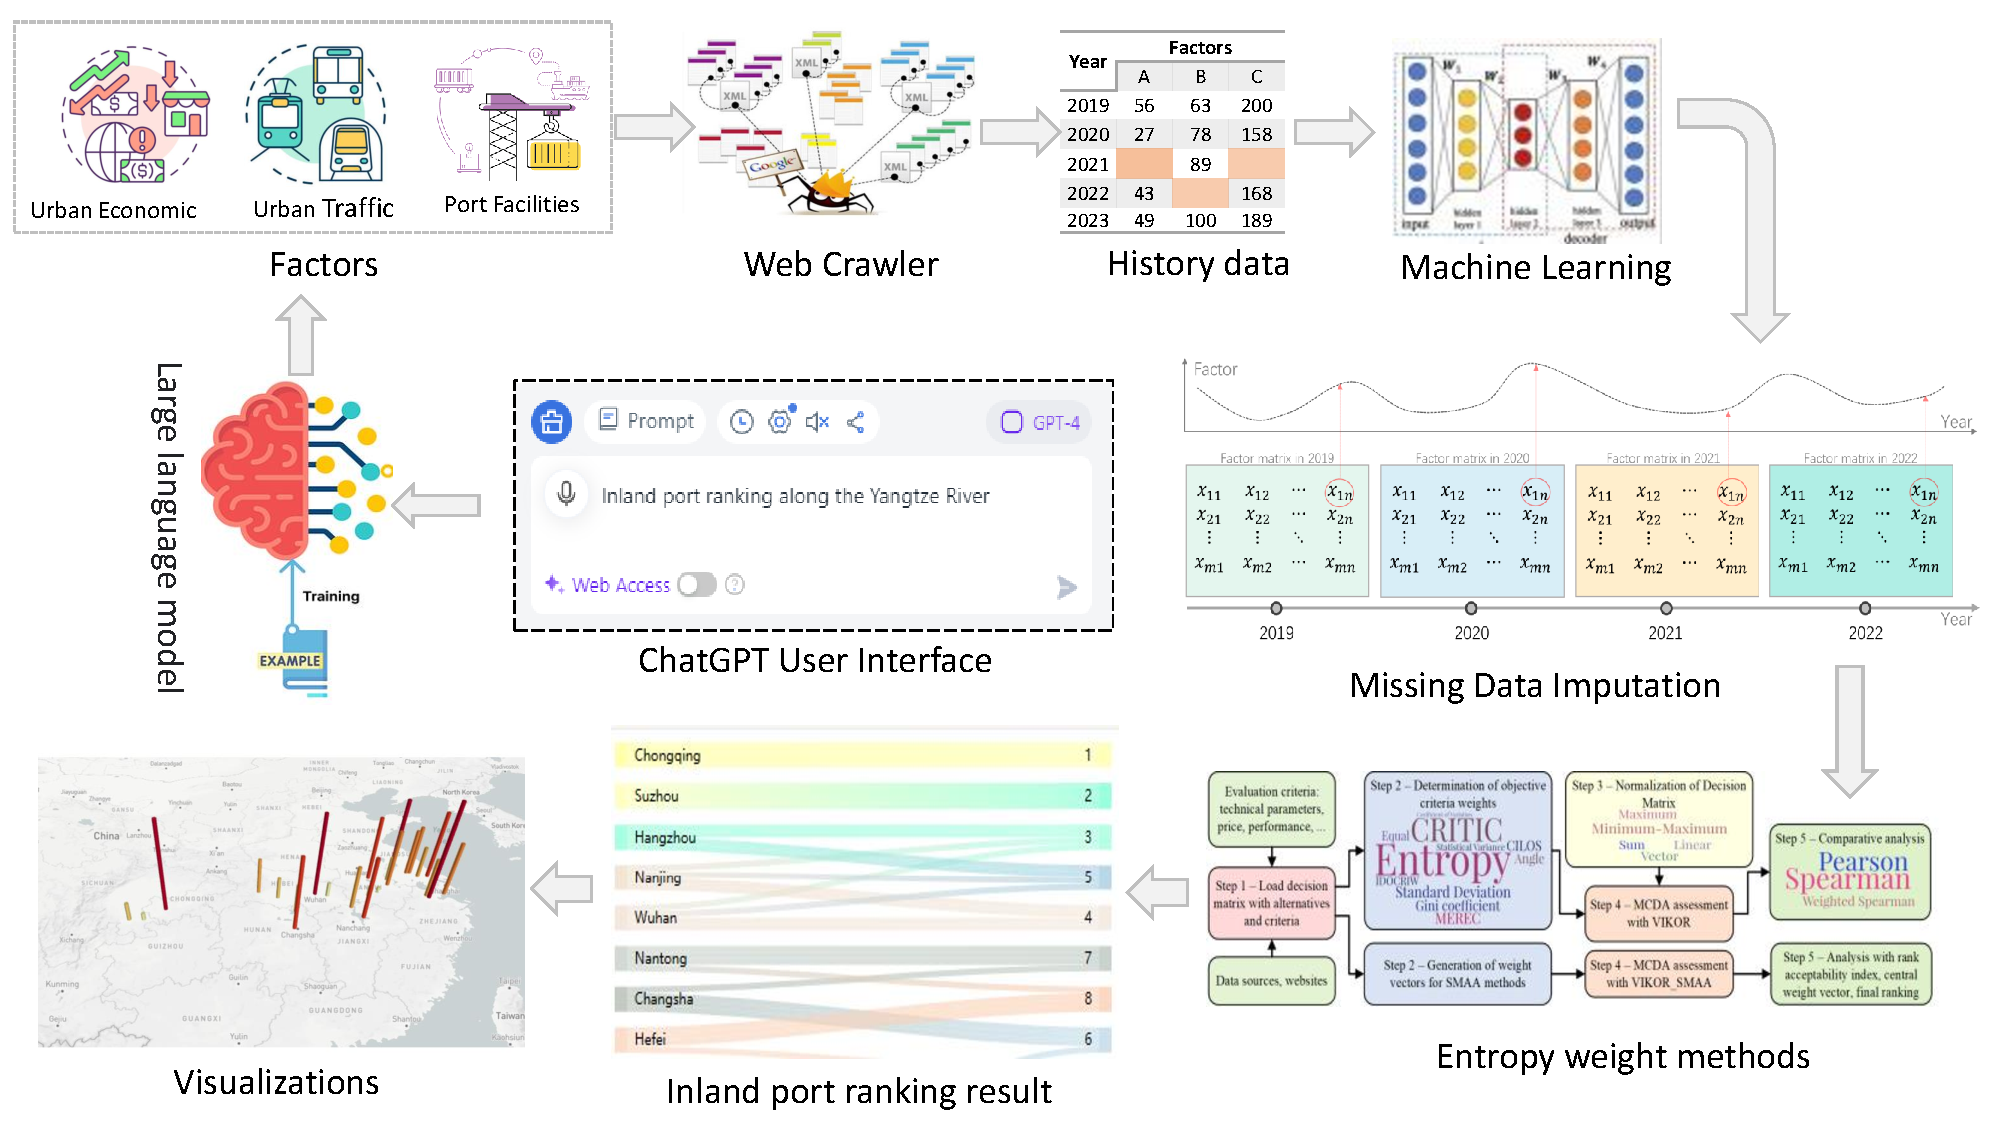
\includegraphics[width=1.0\textwidth]{pic/autoportranking.pdf}
    \caption{Caption}
    \label{fig:enter-label}
\end{figure}
\subsection{Factors}
"Identifying important ports in maritime container shipping networks along the Maritime Silk Road" -When choosing ports to deploy the floating wind with lower cost, H. Díaz  and C. Guedes Soares find ports taht near the wind farms and logistic centers is more efficiently exploit, and deep-water ports with large capacity is better.

"Inland waterway ports nodal attraction indices relevant in development strategies on regional level"
O Dinu1 and others select nodal attraction measures to  find that port ranking varying differently depends on network scales and ccentrality.The research on Danube inland   port also verify that the closer an inland port is to a main road or highway, the better the port development will be.

"An Evaluation of Constituent Factors for Port Logistics" -Aiming at increaseing competitiveness of container ports and improving Korean port container throughput ranking, Gitae Yeo and others use the AHP(Analytic Hierarchy Process) method to evaluate weight and priority values for port logistics from'inner consisted factors' and 'outer requested factors', revealing that, for inner consisted factors, 'information system of port logistics' and handling system' are as priority and the logistics cost is the most important factor among the oter requested factors.

An Analytic Hierarchy Process (AHP) Approach to Port Selection Decisions - Empirical Evidence from Nigerian Ports-About studying the factors when shippers select a port,CHINONYE UGBOMA1 conducted a survey to identify seven criteria for port selection,and used AHP to assess what port criteria are more preferred by shippers, revealing that, comprehensively, shippers attach more importance to efficiency, frequency of ship visits, and for the most preferred port LPC,location account for a quater.

"Port Competitiveness Evaluation Research based on combined model of Cluster and TOPSIS analysis"-The paper combines model of Cluster and TOPSIS analysis to evaluate port competitiveness of ten Chinese seaport, in clulding factors such as customs clearance efficiency and average layover time,Port modernization  management level like EDI system,safety monitoring system and GPS system,port average throughput growth rate, earnings per share and whole image and so on.

% 
"Structures of port connectivity, competition, and shipping networks in Europe"-This paper rank Based on the liner service networks of China-Europe and intra-Europe, the connectivity levels of 29 major European ports with respect to their China-connection centrality levels and intra-Europe centrality levels were evaluated. This shows that the largest European ports are the most "centrally" positioned for both China-Europe network (a transoceanic network) and intra-Europe network (a regional network).

"Dry port location selection using a fuzzy AHP-BWM-PROMETHEE approach"-Mohammed Mojahid Hossain Chowdhury \& Ziaul Haque Munim find out that the distance between the dry port and the exporter or importer,is the crucial for establishing a dry port in Bangladesh.

"The Optimal Location of Dry Port: A Case Study of the Hinterland of Western Side of the Taiwan Straits Port Group"-Ying WANG and Jian WANG established an evaluation index with factors which will affect the development dry port, including Execution efficiency of dry port(customer satisfaction) and transport infrastructure (number of highway and railways linked to the port, Volume of regional freight transportation)
% 
% 
% 
% 
% 
% 
% 
% 
\section{LLM Full Stack Solution for Port Ranking}
\begin{figure}[H]
    \centering
    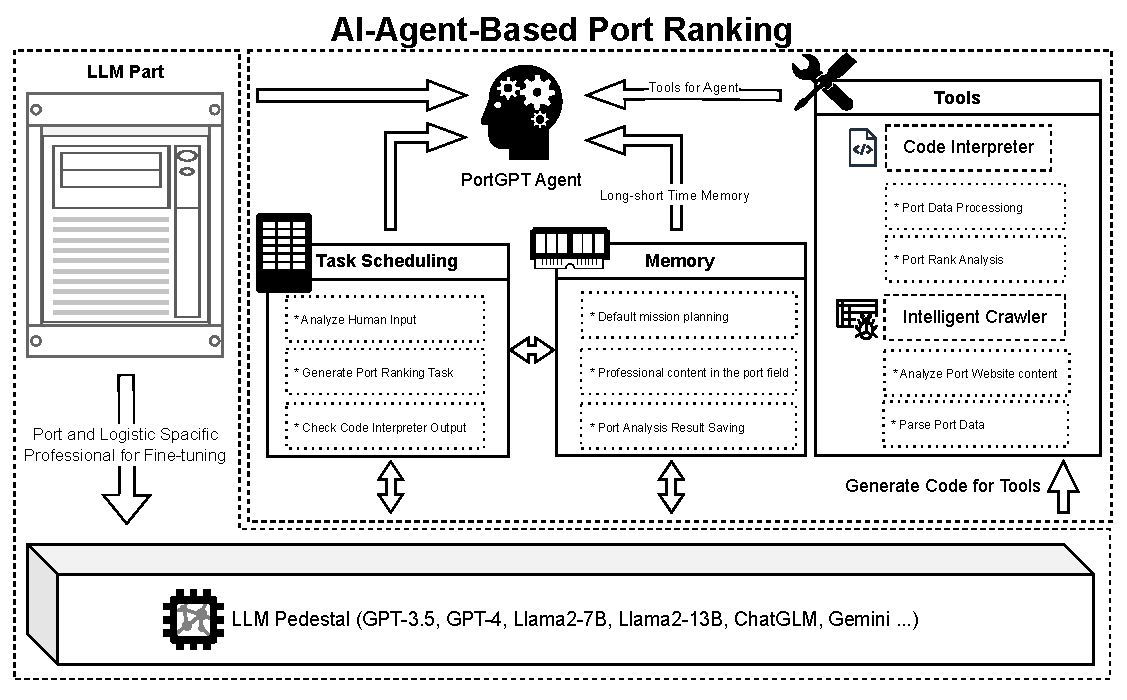
\includegraphics[width=1.0\textwidth]{pic/PortGPT.pdf}
    \caption{PortGPT Conceptual Architecture}
\end{figure}
% 
% 
% 
\subsection{Data collection}
% 
Data Source and Method of Collection
% 
\subsection{Missing Data imputation}
% 
% 
% 
% 
\cite{SUN2023120201}
% 
% 
% 
% 
% 
% 
% 
% 
% 
% 
% 
% 
% 
% 
% 
% 
% 
% 
% 
% 
% 
% 
% 
% 
% 
% 
% 
% 
% 
% 
% 
% 
% 
% 
% 
% 
% 
% 
% 
% 
% \subsection{Data collection}
% 
% \subsection{Missing Data imputation}
% \subsubsection{Fitting of missing data }

% \subsection{Entropy weight method}

% \subsection{Ranking result analysis}
% \subsection{Visualization of results}
% \section{Conclusions}
% 
% 
% 
% 
% 
% 
% 
% 
% 
% 
% 
% 
% 
\bibliographystyle{unsrt}
\bibliography{References}
% 
% 
% 
% 
% 
\end{document}
